\chapter{Pontos Flutuantes}
\label{chap:floatingpoints}

\section{Sistemas de Numeração}
Na matemática, um sistema de numeração consiste em é um conjunto de símbolos e
um esquema ou regra para combiná-los, utilizados para representar quantidades
através do que chamamos de números. Existem dois tipos principais de sistemas:
os posicionais e os aditivos.

O sistema aditivo é aquele em que os números são representados pelas somas dos
valores dos símbolos, geralmente agrupados lado a lado em ordem decrescente,
como, por exemplo, os sistemas romano e egípcio. Já o sistema posicional leva
em conta não só os dígitos mas também a posição que eles ocupam no número. A
quantidade de símbolos diferentes que são utilizados para representar os
dígitos está ligada à \textbf{base} desse sistema, e cada posição do dígito no
número refere-se a uma potência dessa base. Por exemplo, no sistema decimal
(base 10), usamos os dígitos de 0 a 9. No sistema binário (base 2), usamos os
dígitos 0 e 1. E já no sistema hexadecimal (base 16), usamos de 0 a 9 e as
letras A a F (que representam 10 a 15). A quantidade de símbolos diferentes que
são utilizados para representar os dígitos está ligada à \textbf{base} desse
sistema, e cada posição do dígito no número refere-se a uma potência dessa
base. Por exemplo, no sistema decimal (base 10), usamos os dígitos de 0 a 9. No
sistema binário (base 2), usamos os dígitos 0 e 1. E já no sistema hexadecimal
(base 16), usamos de 0 a 9 e as letras A a F (que representam 10 a 15).

Com essas diferentes formas de representar um número, a escolha do sistema
depende do contexto e da aplicação. No uso cotidiano, a base decimal é a mais
utilizada. Já as bases binária e hexadecimal, são amplamente utilizadas na
ciência da computação em operações aritméticas dos processadores e em algumas
linguagens de programação para endereçamento de memória.

Um número $N$ pode ser representado em uma base \(b\) no seguinte formato
\begin{equation}
  N = \pm \sum_{i=-k}^{n} d_i b^i,
\end{equation}
em que \(d_i\) são os dígitos na base \(b\), \(k\) é o número de casas decimais à direita do ponto, e \(n+1+k\) é o número de dígitos significativos. Vejamos alguns exemplos.

\begin{ex}
  Vamos escrever o número 13 nas bases 10 e 2.
  \begin{itemize}
    \item Número na base decimal: $ 13 = 1 \times 10^1 + 3 \times 10^0 = 13_{10}$
    \item Número na base binária: $ 13 = 1 \times 2^3 + 1 \times 2^2 + 0 \times 2^1 + 1
            \times 2^0 = 1101_2$
  \end{itemize}
\end{ex}

\begin{ex}
  Agora vamos escrever o número 3,5625 nas bases 10 e 2.

  \begin{itemize}
    \item Número na base decimal:
          \[
            3{,}5625 = 3 \times 10^0 + 5 \times 10^{-1} + 6 \times 10^{-2} + 2 \times 10^{-3} + 5 \times 10^{-4} = 3{,}5625_{10}
          \]

    \item Número na base binária:
          \[
            3{,}5625 = 1\times 2^{1} + 1 \times 2^0 + 1 \times 2^{-1} + 0 \times 2^{-2} + 0 \times 2^{-3} + 1 \times 2^{-4} = 11{,}1001_2
          \]
  \end{itemize}
\end{ex}

\section{Aritmética de Ponto Flutuante}

A \textit{aritmética de ponto flutuante} é o sistema adotado por computadores
para que lidem com números reais utilizando uma notação compacta e eficaz. Essa
técnica é utilizada para representar e manipular números reais de forma prática
e eficiente. Ela permite representar números de grandezas diversas, que não
podem ser armazenados com precisão, utilizando apenas números inteiros.

Um sistema de ponto flutuante $F$ pode ser definido como
\[
  \mathcal{F}(\beta, t, L, U)\]
cuja representação normalizada de um número real N nesse sistema é dada por
\begin{equation}
  \label{eq:normalizedfp}
  N = \pm (d_{1},d_{2} . . . d_{t})_{\beta} \times \beta^e
\end{equation}
em que
\begin{itemize}
  \item \( N \) é o número real;
  \item \(\beta\) é a base que a máquina opera;
  \item \( t \) é o número de dígitos na mantissa, tal que \( 0 \leq d_{j} \leq \beta-1 \), j = 1, \ldots, t, \(d_{1} \neq 0\);
  \item \( L \) é o menor expoente inteiro;
  \item \( U \) é o maior expoente inteiro;
  \item \( e \) é o expoente inteiro no intervalo [\( L \),\( U \)].
\end{itemize}

\subsection{Representação de Números Reais em Sistemas de Ponto Flutuante}

Em máquinas que operam em sistemas de ponto flutuante, apenas um subconjunto
\textbf{finito} de $\mathbb{R}$ pode ser representado de maneira exata. Por
isso, frequentemente, é necessário limitar a quantidade de dígitos
significativos na representação de números a fim de adequá-los ao sistema que a
máquina opera.

O subconjunto $\mathcal{G} \subset \mathbb{R}$ definido como
\[
  \mathcal{G} = \left\{ \mathcal{F}(\beta,t,L,U)={\pm 0.m \times \beta^e \mid m \in \mathbb{Z}, \beta^{t-1} \le m < \beta^t, L \leq e \leq U}\cup{0} \right\}
\]
é o conjunto dos números que são representáveis pelo sistema $\mathcal{F}$. No conjunto $\mathcal{G}$, apenas alguns números podem ser representados com
precisão, analisemos as seguintes situações para um número real qualquer:

Dado um número real $x$, as seguintes situações podem ocorrer:

\subsubsection*{Caso 1: \( x \in G \) (Número representável)}
Seja $x = 12237,76$. Na forma normalizada temos \(x = 1,223776 \times10^4\). Porém, esse número não pode ser representado precisamente no sistema $F$ e, portanto, precisamos aplicar uma das técnicas de aproximação. Utilizando o truncamento o resultado é \( \bar{x} = 1{,}22377 \times 10^4 \). Já com o arredondamento \( \bar{x} = 1{,}22378 \times 10^4 \).

O número está dentro da faixa de expoente permitida e é representável com perda
controlada de precisão.

\subsubsection*{Caso 2: \( |x| < m \) (Underflow)}
Seja \( x = 0{,}582 \times 10^{-6} \). O expoente é \(-6\) , menor que o limite inferior $L = -5$. Portanto, o número não pode ser representado e ocorre \textbf{underflow}. Nesse caso, na maioria das vezes o valor é tratado como zero.

\subsubsection*{Caso 3: \( |x| > M \) (Overflow)}
Seja \( x = 0{,}927 \times 10^6 \). O expoente é +6, maior que $U = 5$. Portanto, ocorre \textbf{overflow} e o número não pode ser representado precisamente. Neste caso, o valor pode ser tratado como infinito ou como uma flag indicando o \textbf{overflow}.

Devido às limitações da representação de números reais, é necessário empregar
técnicas de aproximação para lidar com números que não podem ser representados
com precisão. Dois dos principais processos empregados para este fim são o
\textbf{truncamento} e o \textbf{arredondamento}.

O truncamento consiste na supressão de todos os dígitos após uma determinada
posição, sem qualquer ajuste adicional no último dígito mantido. Formalmente,
dado um número real \( x \), sua aproximação truncada com \( n \) dígitos na
base \( b \) é expressa por
\[
  T(x) = \sum_{i = -k}^{n-1} d_i b^i
\]
onde os dígitos \( d_i \) com \( i < -k \) são descartados.

O erro introduzido por este processo, dado por $E_T = x-T(x)$, é denominado
\textit{erro de truncamento}. Ele é limitado superiormente pela base elevada à
potência negativa do número de dígitos mantidos, ou seja, $|x - T(x)| <
  b^{-k}$.

\begin{ex}
  Considere a aproximação com oito casas decimais de \(\pi = 3,14159265\).
  Para truncar $\pi$  com precisão de 4 casas decimais, descartamos todos os termos da sexta casa em diante. Assim, o valor truncado fica
  $T(\pi) = 3,1415$.
  O erro do truncamento é, nesse caso, $E_T = 3,14159265 - 3,1415 = 0,00009265$. Diante disso, podemos observar que $|E_T| < 10^{-4}$.
\end{ex}

O arredondamento, por outro lado, ajusta o último dígito mantido com base no
valor do primeiro dígito descartado, buscando minimizar o erro absoluto da
aproximação. No arredondamento simétrico (ou clássico), se o primeiro dígito
descartado for maior ou igual a \( \frac{b^{-n}}{2} \), incrementa-se o último
dígito mantido em uma unidade; caso contrário, seu valor permanece inalterado.

Seja \( x \) um número real e \( R(x) \) sua aproximação arredondada com \( n
\) dígitos na base \( b \). O erro de arredondamento satisfaz $|x - R(x)| \leq
  \frac{1}{2} b^{-n}$

\begin{ex}
  Ainda considerando a mesma aproximação de \(\pi = 3,14159265\).
  Para arredondar $\pi$  com precisão de 4 casas decimais, vamos analisar o número da próxima casa em que queremos arredondar. Nesse caso, o número na quinta posição é 9, então vamos arredondar a quarta casa para cima $R(\pi) = 3,1416$. O erro do arredondamento é, nesse caso, $E_R = 3,14159265 - 3,1416  = -0,00000735$. Diante disso, podemos observar que $|E_R| \leq  \frac{ 1}{2}10^{-4}$ e consequentemente $|E_R| \leq  |E_T|$.
\end{ex}

Em geral, o erro máximo introduzido pelo arredondamento é metade daquele
introduzido pelo truncamento, razão pela qual o arredondamento tende a produzir
aproximações mais precisas.

Vejamos a seguir uma comparação das técnicas de arredondamento e de
truncamento, considerando uma máquina decimal com 3 dígitos na mantissa e
expoentes variando de –4 a 4:
\begin{center}
  \small
  \begin{tabular}{|c|c|c|c|c|}
    \hline
    \textbf{Número Real} & \textbf{Arredondamento}        & \textbf{\(E_R\)}             & \textbf{Truncamento}       & \textbf{\(E_T\)}             \\
    \hline
    5{,}678              & \( 0{,}568 \times 10^1 \)      & \( 0{,}2 \times 10^{-3} \)   & \( 0{,}567 \times 10^1 \)  & \( 0{,}8 \times 10^{-3} \)   \\
    \hline
    –192{,}73            & \( -0{,}193 \times 10^3 \)     & \( 0{,}27 \times 10^{1} \)   & \( -0{,}192 \times 10^3 \) & \( 0{,}73 \times 10^{1} \)   \\
    \hline
    3{,}14159            & \( 0{,}314 \times 10^1 \)      & \( 0{,}159 \times 10^{-2} \) & \( 0{,}314 \times 10^1 \)  & \( 0{,}159 \times 10^{-2} \) \\
    \hline
    0{,}0000063          & \multicolumn{4}{c|}{Underflow}                                                                                            \\
    \hline
    920000{,}0           & \multicolumn{4}{c|}{Overflow}                                                                                             \\
    \hline
  \end{tabular}
\end{center}

\subsubsection{Representação Especial do Zero e Subnormais}

Na representação de ponto flutuante, um número real é geralmente expresso na
forma normalizada (ver Equação~\ref{eq:normalizedfp}), com \( d_1 \neq 0 \),
garantindo o aproveitamento máximo da precisão disponível e evitando
representações redundantes. Contudo, o número zero não pode ser representado
nesta forma, pois exigiria \( d_1 = 0 \), o que contraria a normalização.

Assim, o zero recebe uma \textit{representação especial} denotada por
\begin{equation}
  N = \pm (0{,}000\ldots 0_{t})_\beta \times \beta^{L - 1},
\end{equation}
em que \( L \) é o menor expoente permitido no sistema. Este tratamento
especial assegura que o zero seja manipulado de forma única e consistente
dentro do sistema de ponto flutuante, evitando, assim, a perda de informação ao
realizar operações aritméticas que o envolvam. Essa perda de informação será
discutida na seção \ref{subsec:erroselim}.

Assim como a representação do zero, existem as representações subnormais, que
são números muito pequenos, com magnitude menor que o menor número normalizado
representável. Eles são expressos na forma
\begin{equation}
  N = \pm (0{,}000\ldots 0_{t})_\beta \times \beta^{L - 1},
\end{equation}

Um exemplo de aplicação para subnormais é no \textit{fade-in} e
\textit{fade-out} de sinais de áudio, em que a amplitude do sinal precisa ser
reduzida gradualmente até zero, evitando cortes abruptos que poderiam gerar
ruídos indesejados. Nesses casos, os subnormais permitem que representar
valores muito pequenos de forma contínua e suave, garantindo uma transição mais
natural e agradável ao ouvido humano.

%\newpage

\subsection{Representação de Pontos Flutuantes em Computadores (Padrão IEEE 754)}
Sistemas eletrônicos, como computadores modernos, utilizam um sistema de ponto
flutuante padronizado, conhecido como IEEE 754, para representar números reais.
Esse padrão foi definido para garantir consistência e precisão na representação
de números em diferentes plataformas e linguagens de programação. Computadores
utilizam a base binária ($\beta= 2$) para representar números, incluindo os
números reais. Então qualquer número nesse sistema é composto pelos algarismos
0 e 1, que também são chamados de bits.

\subsubsection*{Menor e Maior valor num sistema de ponto flutuante}

Para compreendermos melhor as limitações na representação de números em um
sistema de ponto flutuante, vamos explorar o exemplo a seguir. Seja uma máquina
opere no sistema $\mathcal{F}(\beta=10; t=5; L=-5; U=5)$. Nesse sistema, os
números serão representados da seguinte maneira
\begin{equation*}
  \pm (0.d_{1}d_{2} . . . d_{t}) \times 10^e,  0 \leq |d_{j}| \leq 9,  d_{1} \neq 0, e \in [-5,5].
\end{equation*}
O \textbf{menor valor normalizado}, em módulo, representado nesse sistema é
$  m = 0.10000 \times 10^{-5} = 10^{-6},$ enquanto que o \textbf{maior valor } é $M = 0.99999 \times 10^{5} = 99999$.

\subsubsection{Estrutura de um Número de Ponto Flutuante no padrão IEEE 754}

No padrão IEEE 754 \cite{IEEE754} um número de ponto flutuante é dividido em
três partes. O primeiro bit, representa o \textbf{Sinal (S)} do número
representado, indicando se o número é positivo (\( S = 0 \)) ou negativo (\( S
= 1 \)); Os próximos $N$ bits representão o \textbf{expoente (E)} com viés
(bias), que é calculado como $\text{bias} = 2^{(N-1)} - 1$; E por fim, os
últimos $M$ bits representam a \textbf{Mantissa (M)} que é parte fracionária
significativa do número.

A fórmula completa de reconstrução do número é dada por
\[
  x = (-1)^S \times (1.M) \times 2^{E - \text{bias}}
\]

Na mantissa, o termo $1.M$ indica que há um bit implícito ``1'' antes da
mantissa nos números normalizados.
\subsubsection{Nível de Precisão de um Sistema de Ponto Flutuante}

Frequentemente é interessante representar números reais com diferentes níveis
de precisão, dependendo da aplicação envolvida. Para tarefas simples, baixa
precisão pode ser suficiente e gastar menos memória. Já para cálculos mais
complexos, como os envolvidos em simulações científicas, alta precisão é
necessaria para garantir uma representação mais fiel dos números reais e
reduzir o impacto dos erros de arredondamento. Alguns dos sistemas mais comuns
de precisão são \textbf{Meia Precisão (16 bits)}, \textbf{Precisão Simples (32
  bits)}, \textbf{Precisão Dupla (64 bits)} e \textbf{Precisão Quadrupla (128
  bits)} e estão descritos na tabela~\ref{tab:precision}.

\begin{center}
  \small
  \begin{tabular}{lcccc}
    \toprule
    \textbf{Característica}
                     & \textbf{Half}
                     & \textbf{Single}
                     & \textbf{Double}
                     & \textbf{Quadruple}
    \\
    \midrule

    Bits totais      & 16                 & 32              & 64                & 128          \\

    Bit de sinal     & 1                  & 1               & 1                 & 1            \\

    Bits de expoente & 5                  & 8               & 11                & 15           \\

    Bits de mantissa & 10                 & 23              & 52                & 112          \\

    Bias             & 15                 & 127             & 1023              & 16383        \\

    Expoente real    & $-14$ a $+15$      & $-126$ a $+127$ & $-1022$ a $+1023$ & $-16382$
    a $+16383$                                                                                 \\

    Precisão decimal & $\approx 3$        & $\approx 7$     & $\approx 16$      & $\approx 34$ \\

    \bottomrule
    \label{tab:precision}
  \end{tabular}
\end{center}

\begin{ex}

  Considere o número decimal \( x = -12{,}25 \). Sua representação binária é $x =
    -1100{,}01_2 = -1{,}10001000000000000000000 \times 2^3$.

  Façamos então, uma análise dos componentes do número. O número é negativo,
  então o bit Sinal deve ser $s = 1$. A mantissa, sem o bit oculto é
  $10001000000000000000000$, e o expoente real é $e = 3$. Para precisão simples,
  o bias é $127$, então o expoente com bias é $e + \text{bias} = 3 + 127 =
    130_{10}$ conventendo para base binária, temos $130_{10} = 10000010_2$. Então
  representamos o número no padrão IEEE como
  \[
    \begin{array}{|c|c|c|} \hline
      s_n & e        & m                       \\ \hline
      1   & 10000010 & 10001000000000000000000 \\ \hline
    \end{array}
  \]
\end{ex}

Para outras precisões, o processo é análogo, mudando apenas o número de bits e
o bias.

A escolha do tipo de precisão depende muito da aplicação. Em geral, a
\textbf{Precisão Simples} ou \textbf{Meia Precisão} são adequadas para
aplicações com memória limitada e que não exigem alta precisão. Já a
\textbf{Precisão Dupla e Quádrupla} são usadas em aplicações científicas,
cálculos de engenharia, simulações e algoritmos numéricos mais sensíveis.

\section{Erros e Limitações}\label{subsec:erroselim}

Erros em operações com pontos flutuantes podem se propagar e aumentar em
cálculos mais complexos. Por exemplo, pequenos erros de arredondamento em
etapas iniciais podem afetar significativamente o resultado final,
especialmente em somas repetitivas ou subtrações de números muito próximos.
Isso torna importante considerar a ordem das operações e o impacto da precisão
em aplicações sensíveis.

\subsection{Erro Absoluto e Relativo}

Em cálculos numéricos, frequentemente lidamos com aproximações devido a
arredondamentos e truncamentos. Para avaliar a precisão dessas aproximações,
utilizamos as métricas de erro absoluto e erro relativo.

O erro absoluto mede a diferença entre o valor real \(\boldsymbol{x_r}\) e o
valor aproximado \(\boldsymbol{x_a}\), ou seja, a quantidade exata de erro na
aproximação. Ele é definido como:

\begin{equation}
  \text{EA} = |x_a - x_r|.
\end{equation}

Quanto menor for o erro absoluto, mais próximo o valor aproximado está do valor
real. No entanto, essa métrica não fornece informações diretas sobre o impacto
do erro em relação à magnitude do número em questão.

O erro relativo indica o quão preciso é o valor aproximado em relação ao valor
real. Ele pode ser tratado como um decimal ou na forma de porcentagem. Ele é
definido como
\begin{equation}
  \text{ER} = \frac{|x_a - x_r|}{|x_r|}\ \ \textrm{ou}\ \ \frac{|x_a - x_r|}{|x_r|}\times 100\%.
\end{equation}
Isso pode ser reescrito como
\begin{equation}
  \text{ER} = \frac{{EA}}{|x_r|}\ \ \textrm{ou}\ \ \frac{{EA}}{|x_r|}\times 100\%.
\end{equation}
Essa métrica é útil quando lidamos com valores de grandezas muito diferentes. Por exemplo, um erro absoluto de \( 0.1 \) pode ser insignificante se estivermos tratando de números na ordem de milhares, mas pode ser relevante se estivermos lidando com valores decimais.

Vamos analisar dois casos com mesmo erro absoluto mas diferentes erros
relativos. Considere um valor real \( x_{r1} = 10.5 \) com uma aproximação de
\( x_{a1} = 10.3 \). O seu erro absoluto é \(|10.3 - 10.5| = 0.2\) e seu erro
relativo \(\frac{0.2}{10.5} \approx 0.019\) (ou 1.9\%). Agora considere um
segundo valor real de \(x_{r2} = 0.4 \) com uma aproximação de \(x_{a2} = 0.2
\), seu erro absoluto é \(|0.4 - 0.2| = 0.2\), o seu erro relativo será
\(\frac{0.2}{0.4} = 0.5\) ou seja, 50\%.

\begin{center}
  \small
  \begin{tabular}{|c|c|c|c|}
    \hline
    \textbf{Número Real} & \textbf{Aproximação} & \textbf{Erro Absoluto} & \textbf{Erro Relativo}          \\
    \hline
    \(  10{.}5 \)        & \(  10{.}3 \)        & \(  0{.}2 \)           & \(  0{.}019 \) ou \( 1{.}9\% \) \\
    \hline
    \(  0{.}4 \)         & \(  0{.}2 \)         & \(  0{.}2 \)           & \(  0{.}5 \) ou \( 50{.}0\% \)  \\
    \hline
  \end{tabular}
\end{center}
Apesar dos dois casos terem o mesmo erro absoluto \( (EA=  0{.}2) \), o erro relativo relacionado à aproximação no primeiro caso representa menos de 2\% do valor real, indicando que a aproximação é razoavelmente precisa. Em contrapartida, no segundo caso, o erro relativo é de 50\%, um valor relativamente alto comparado ao primeiro, o que indica uma aproximação deficiente. Dessa forma, o erro relativo é uma ferramenta importante para interpretar melhor a qualidade de uma aproximação, independentemente da escala dos números envolvidos.

\section{Perda de Significância em Operações com Pontos Flutuantes}
A perda de significância (também conhecida como cancelamento catastrófico)
ocorre de modo mais evidente quando há grande diferença de ordem de grandeza
entre os números envolvidos na operação. Por exemplo, considere:

\[
  x = 1{,}000 \times 10^{4} \quad \text{e} \quad y = 0{,}276 \times 10^{-2}.
\]

Para realizar a soma, ambos os operandos precisam ser expressos com o mesmo
expoente:

\[
  x = 1{,}000000000 \times 10^4, \quad y = 0{,}000000276 \times 10^4.
\]

A soma exata seria:

\[
  x + y = (1{,}000000000 + 0{,}000000276) \times 10^4 = 1{,}000000276 \times 10^4.
\]

Contudo, devido à precisão limitada do sistema (7 dígitos significativos), a
aritmética de ponto flutuante armazena apenas:

\[
  x + y \approx 1{,}0000002 \times 10^4.
\]

Uma parte do termo \( y \) é completamente desprezada, e a soma não resulta
numericamente igual a \( x + y\), evidenciando a perda catastrófica de
significância.

Outro caso peculiar é a soma de um número muito grande com uma sequência de
números pequenos. Dependendo da ordem em que as somas são realizadas, o número
grande pode "mascarar" os pequenos, resultando em diferentes valores finais.

Por exemplo:
\[
  S = 10^{8} + 10^{-1} + 10^{-2} + 10^{-3} + \ldots + 10^{-10}.
\]
Se somarmos primeiro o número grande (\(10^8\)) e depois os números pequenos,
muitos destes podem ser ignorados devido à falta de precisão da mantissa. Por
outro lado, ao somar os números pequenos antes, o valor final será mais próximo
do esperado.

Para ilustrar, suponha a seguinte ordem de cálculo:
\begin{itemize}
  \item Caso 1: \(S = 10^{8} + (10^{-1} + 10^{-2} + \ldots + 10^{-10})\).
  \item Caso 2: \(S = (10^{-1} + 10^{-2} + \ldots + 10^{-10}) + 10^{8}\).
\end{itemize}
No primeiro caso, muitos números pequenos são ignorados devido ao arredondamento. No segundo, o somatório dos números pequenos é calculado antes de adicionar o número grande, preservando mais informações significativas.

\subsubsection*{Prevenção da perda de significância em operações com Zero}
\label{subsec:repZero}

O zero possui uma representação especial na aritmética de ponto flutuante
devido à sua importância nas operações numéricas e à necessidade de evitar
ambiguidades. Essa representação permite o tratamento adequado de operações que
envolvem valores nulos, prevenindo erros numéricos e a perda de significância
em cálculos sensíveis. Considere um sistema de ponto flutuante \( F(10, 7, -5,
5) \). Sejam
\[
  x = 0{,}000 \times 10^{-6} \quad (\text{o número zero}), \quad y = 0{,}276 \times 10^{-2}.
\]
Na operação de soma:
\[
  x + y = 0{,}276 \times 10^{-2},
\]
como \( x \) é exatamente zero, o resultado mantém integralmente os dígitos
significativos de \( y \). Se o zero não tivesse uma representação especial e
fosse tratado como um número subnormal com expoente mínimo, o alinhamento das
mantissas poderia comprometer a precisão de \( y \), deslocando seus dígitos
significativos e resultando em perda de informação. Nesse sentido, suponha que
\( x \) não tivesse uma representação especial e fosse tratado como um número
subnormal com o expoente mínimo \( -5 \), com mantissa ajustada para
\[
  x' = 0{,}000000 \times 10^{-5}.
\]
Para somar \( x' \) e \( y \), é necessário alinhar os expoentes, o que implica
deslocar a mantissa de \( y \) para a direita:
\[
  y = 0{,}276 \times 10^{-2} = 0{,}00000276 \times 10^{-5}.
\]
Ao realizar a soma,
\[
  x' + y = (0{,}000000 + 0{,}00000276) \times 10^{-5} = 0{,}00000276 \times 10^{-5}.
\]
Devido à precisão limitada do sistema (7 dígitos significativos), essa operação
pode fazer com que os dígitos significativos de \( y \) sejam deslocados para
posições menos precisas, causando perda de informação relevante.
\[
  x' + y = 0{,}0000027 \times 10^{-5}.
\]

Portanto, a representação especial do zero evita esse problema, preservando a
precisão e assegurando a estabilidade numérica das operações.

\section{Análise de Instabilidades e Casos Peculiares}
Na aritmética de ponto flutuante, certos casos resultam em erros devido à
limitação da precisão e à maneira como os números são representados.

\subsection{Units in Last Place (ULP's)}
Diferentemente dos conjuntos matatemáticos comuns ($\mathbb{R}, \mathbb{Z}$,
etc.), todo conjunto de números de um sistema de ponto flutuante (PF) é, por
natureza, discreto, ou seja, possui uma quantidade finita de números
representáveis. Para cada número real $x$ existe um $X$ que será a sua
representação num dado sistema de PF. As ULP's foram inicialmente introduzidas
em 1960 por William Kahan, que definiu $ulp(x)$ pela lacuna entre dois números
$X_{1}$ e $X_{2}$ mais próximos de $x$, mesmo que $x$ seja um deles. Tome o
sistema $\mathcal{F}(\beta = 2; t = 3; L = 3 ; U = 5)$. O menor número que pode
ser representado nesse sistema é $1{,}00_{2}$ x $2^{3}$ = $8_{10}$, o seu
sucessor é $1{,}01_{2}$ = $1{,}25_{10}$ x $2^{3}$ = $10_{10}$. Em $x \in
  [8_{10} , 10_{10}]$ ulp ($x$) = 2, ou seja, não é possível representar nenhum
número entre 8 e 10 nesse sistema.

Para definir para qual PF $x$ o número real $x$ será aproximado, existem várias
estratégias, como o truncamento e o arredondamento. A escolha da estratégia de
aproximação pode afetar o valor de ulp($x$). Por exemplo, se $x = 9{,}6_{10}$,
no sistema $\mathcal{F}(\beta = 2; t = 3; L = 3 ; U = 5)$, o valor de ulp($x$)
é 2. Se usarmos truncamento, $X = 8_{10}$ e o erro absoluto é $|x - X| =
  1{,}6_{10}$, ou seja, $0{,}8 \times ulp(x)$. Se usarmos arredondamento, $X =
  10_{10}$ e o erro absoluto é $|x - X| = 0{,}4_{10}$, ou seja, $0{,}2 \times
  ulp(x)$.

Com o passar do tempo, a adoção do padrão IEEE 754, lidar com infinitos e
\textit{Not a Number (NaN's)} tornou-se uma tarefa necessária, o que exigiu um
redefinição $\mathrm{ulp}(x)$ como a lacuna entre dois números $X_{1}$ e
$X_{2}$ mais próximos de $x$, mesmo que $x$ seja um deles. E em particular,
$\mathrm{ulp}(\mathrm{NaN}) = \mathrm{NaN}$.

Para fins práticos, podemos calcular a ULP de um número real $x$ com expoente
real $e$ e $t$ digitos significativos a partir da seguinte expressão
\begin{equation}
  ULP(x) = \beta^{e - t + 1}.
  \label{eq:ulp}
\end{equation}

\begin{ex}
  Por exemplo, considere o número $5.5^{23}$. Para representá-lo em ponto flutuante de precisão dupla (64 bits), primeiro precisamos determinar o expoente binário
  do número. Isso pode ser feito observando entre quais potências de 2 o valor se
  encontra.

  Utilizando uma calculadora para achar uma aproximação do número, temos:$
    5.5^{23} \approx 8.18545 \times 10^{16}.$ Comparando com potências de 2 mais
  próximas, $2^{56} \approx 7,2 \times 10^{16}$ e $ 2^{57} \approx 1,4 \times
    10^{17}$, percebemos que $2^{56} < 5.5^{23} < 2^{57}$, dessa forma o número
  pode ser escrito na forma normalizada em base 2 $5.5^{23} = (1.f) \times
    2^{56}$, assim, o expoente real é e = 56.

  Em precisão dupla, o expoente armazenado utiliza um \textit{bias} de 1023,
  portanto $E = e + 1023 = 56 + 1023 = 1079$. Resta calcular a mantissa,
  normalizando o número

  \begin{align*}
    1.f & = \frac{5.5^{23}}{2^{56}}                                \\
    1.f & \approx \frac{8.18545 \times 10^{16}}{72057594037927936} \\
        & \approx 1.135905
  \end{align*}
  Temos que $f \approx 0.135905$, portanto, a representação normalizada aproximada do número é $5.5^{23} \approx (-1)^0 \times (1.135905) \times 2^{56}$.

  O erro de ponto flutuante pode ser definido como a diferença entre o valor real
  e o valor representado em ponto flutuante, $ Erro = \left|\bar{x} - x\right|$.

  O número $5.5^{23}$ é um número muito grande, e quando representado em ponto
  flutuante, ele pode ser aproximado para um valor próximo a $1.0 \times
    10^{16}$.

  Ainda considerando uma precisão dupla, a ULP para o número $5.5^{23}$ pode ser
  calculada por
  \begin{align*}
    ULP(5.5^{23}) & = 2^{e - t + 1}
                  & = 2^{56 - 53 + 1}
                  & = 2^{4} = 16.
  \end{align*}

\end{ex}
O gráfico da função $ulp(x^{23})$ para um sistema IEEE 754 de precisão dupla ,representado na Figura~\ref{fig:func_ulp}, ilustra como a ULP cresce à medida que o valor de $x^{23}$ aumenta.
\begin{figure}[h]
  \centering
  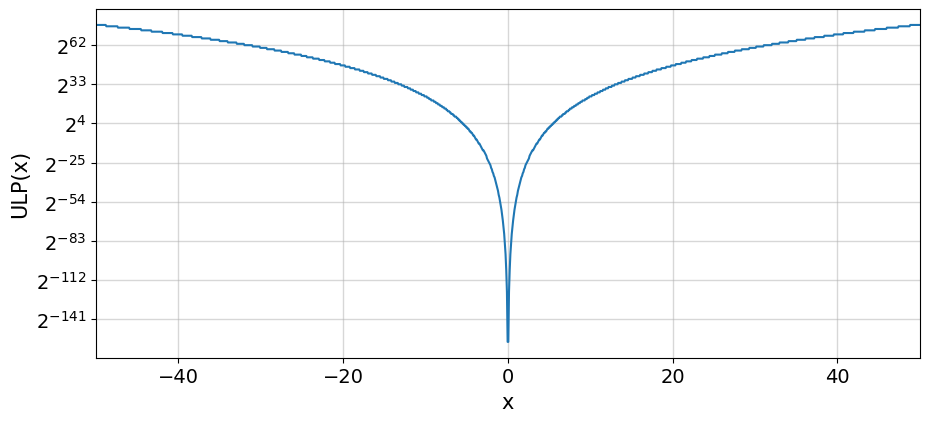
\includegraphics[width=.9\textwidth]{Imagens/ulps/ulp2}
  \caption{Função $ulp(x^{23})$ num sistema IEEE 754 de precisão dupla.}
  \label{fig:func_ulp}
\end{figure}

\subsection{Imprecisão de operações em Sistemas de Ponto flutuante}
Considere o cálculo de $f(x) = x^{10} + 1 - x^{10}$ para \(x \in [-60, 60]\).
As partes envolvendo $x$ são variáveis e a parte ``$1$'' é o literal, ou seja,
um valor fixo. Embora para $x \in \mathbb{R}$ o resultado de $f(x)$ seja igual
a 1, ao efetuarmos os cálculos usando ponto flutuante, observamos um
comportamento inesperado em que o valor correto é exibido apenas até um certo
valor de $x$. Após esse valor observamos um intervalo em que ocorre uma
oscilação no resultado da função e, em seguida, observamos que a função assume
o valor zero, como ilustrado na Figura~\ref{fig:catastrofic_cancelation}
e~\ref{fig:zoom}.

\begin{figure}[h]
  \centering
  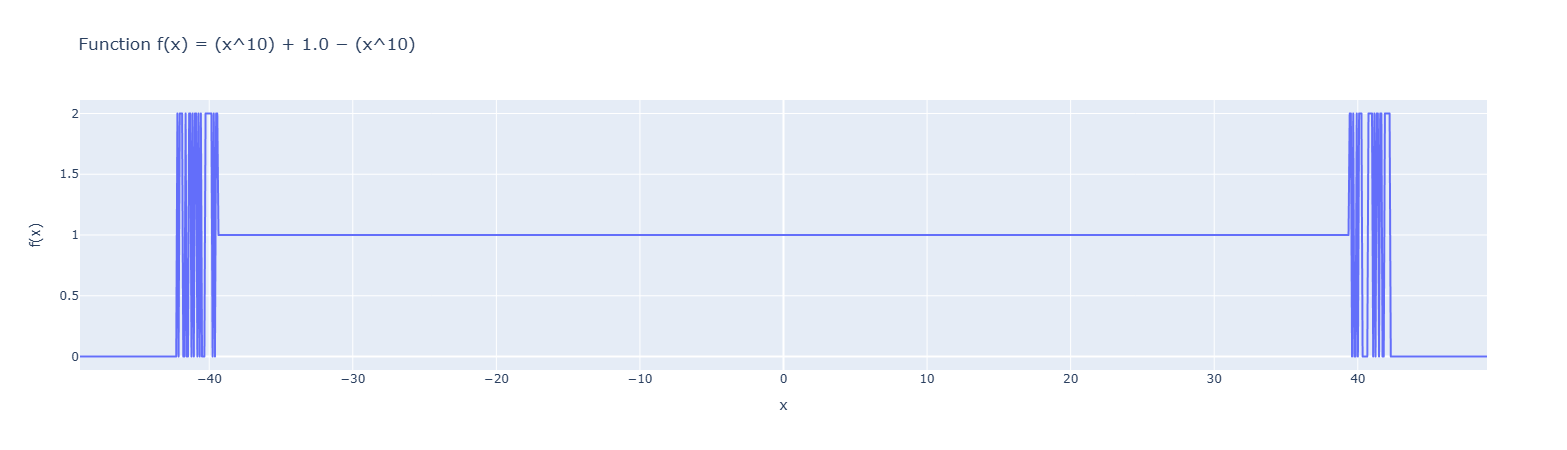
\includegraphics[width=1\textwidth]{Imagens/casosPeculiaresFP/catastrofic_cancelation.png}
  \caption{Comportamento da expressão \(x^{10} + 1 - x^{10}\) no intervalo \([-40, 40]\).}
  \label{fig:catastrofic_cancelation}
\end{figure}
\begin{figure}[h]
  \centering
  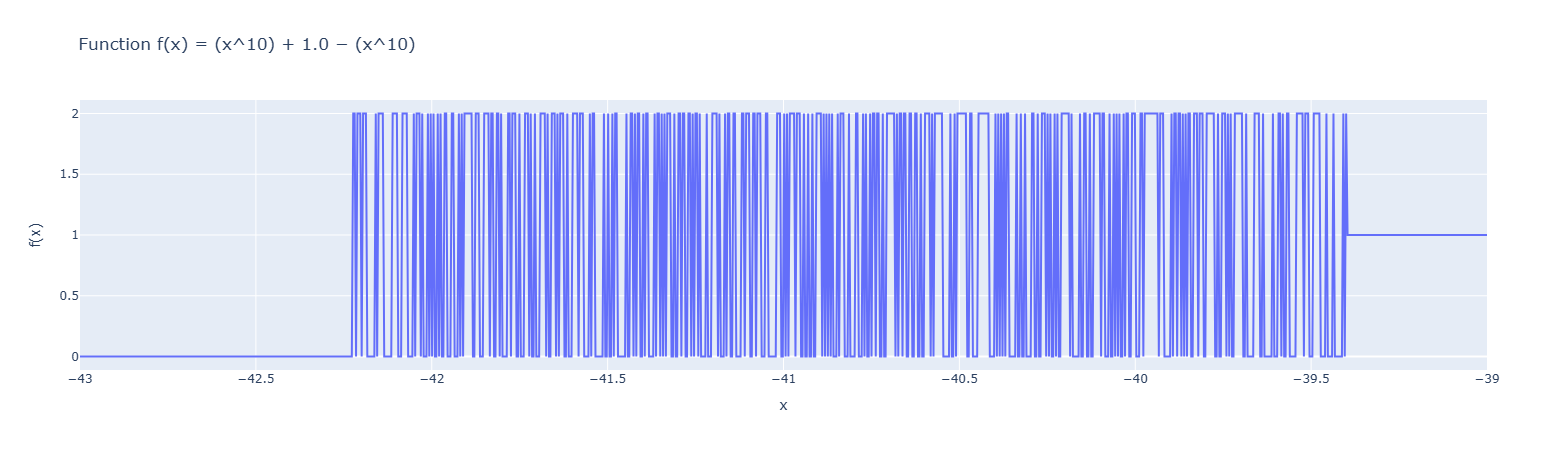
\includegraphics[width=1\textwidth]{Imagens/casosPeculiaresFP/zoom.png}
  \caption{Comportamento da expressão \(x^{10} + 1 - x^{10}\) no intervalo \([-43, -39]\).}
  \label{fig:zoom}
\end{figure}

A partir de um determinado limiar, a função para de se comportar como esperado
$f(x) = 1$ e passa a assumir valores os de $f(x) = 2$ e $f(x) = 0$. Vamos
manipular essa expressão e ver como ela se comporta em diferentes situações.

\begin{figure}[h]
  \centering
  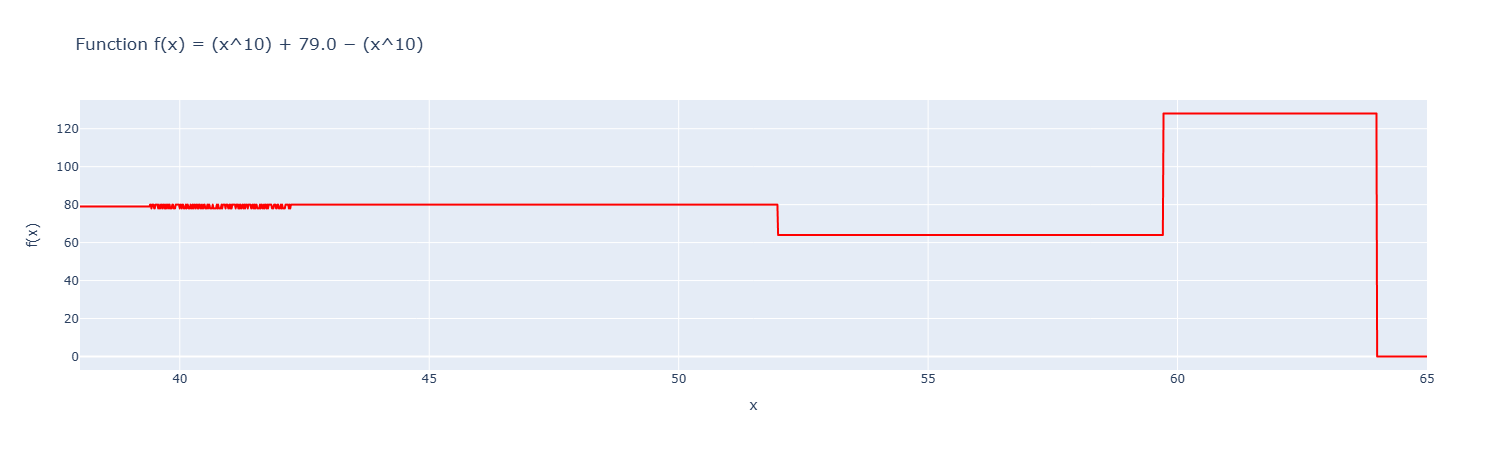
\includegraphics[width=1\textwidth]{Imagens/casosPeculiaresFP/literal79.png}
  \caption{Comportamento da expressão \(x^{10} + 79 - x^{10}\) no intervalo \([38, 65]\).}
  \label{fig:literal79}
\end{figure}

Na figura \ref{fig:literal79}. é possível observar que a função assume mais de
dois valores inesperados para $f(x)$, nesse caso, o conjunto imagem no
intervalo \([38, 65]\) é \( Im(f) = \bigl\{ {0{,}64{,}78{,}79{,}80{,}128}\}\).
O seguinte conjunto de valores para o literal foi testado \(\{3,12,79,98\}\), e
hipotetiza-se que para valores que não podem ser escritos como uma potência de
base 2, esse padrão ocorra.

Uma dúvida comum é se a precisão desses sistemas afeta nessa expressão. Vamos
comparar então um sistema de float32 (Cerca de 7-8 bits dígitos decimais de
precisão) a um sistema float64 (Cerca de 15-16 dígitos decimais de precisão)
\begin{figure}[h]
  \centering
  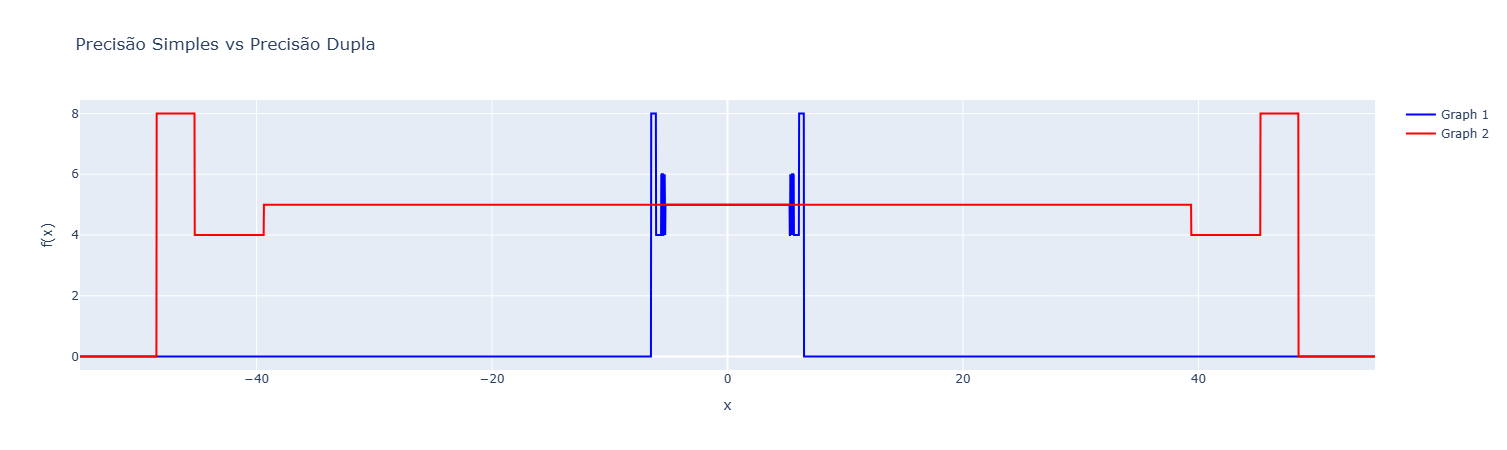
\includegraphics[width=1\textwidth]{Imagens/casosPeculiaresFP/32x64_full.png}
  \caption{Comportamento da expressão \(x^{10} + 2 - x^{10}\) no intervalo \([-40, 40]\).}
  \label{fig:32x64_full}
\end{figure}
\begin{figure}[H]
  \centering
  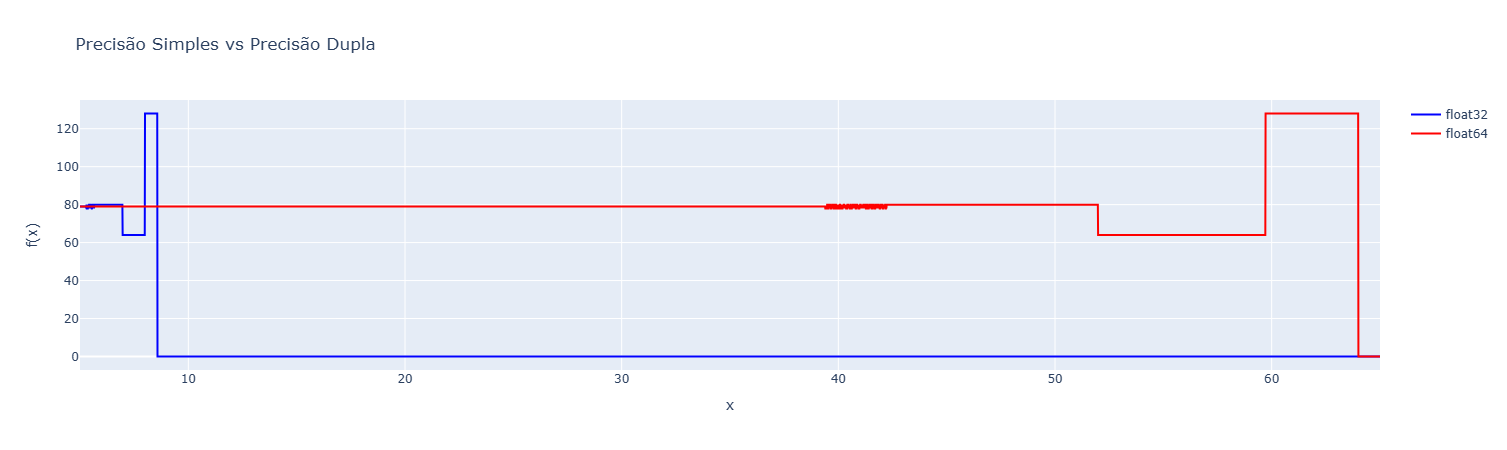
\includegraphics[width=1\textwidth]{Imagens/casosPeculiaresFP/32x64.png}
  \caption{Comportamento da expressão \(x^{10} + 79 - x^{10}\) no intervalo \([0, 60]\).}
  \label{fig:32x64}
\end{figure}
Dos testes experimentais, exemplificado nas figuras \ref{fig:32x64_full} e \ref{fig:32x64}, foi concluído que o $|x|$ onde a instabilidade ocorre é menor é menor na precisão dupla.

Outro caso interessante é quando analisamos a função $f(x) = (x\times x\times
  x\times x\times x\times x\times x\times x \times x) - x^{10} $. Vejamos o
gráfico dessa função.
\begin{figure}[H]
  \centering
  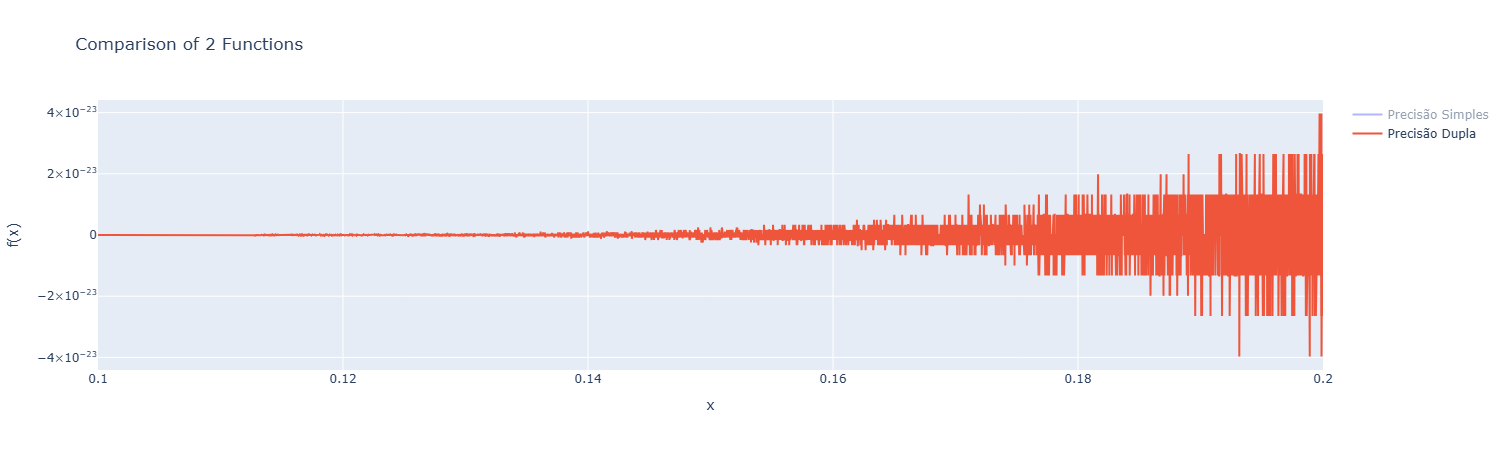
\includegraphics[width=1\textwidth]{Imagens/casosPeculiaresFP/timesXpot_literal0.png}
  \caption{Comportamento da expressão $f(x) = (x \times x \times x \times x \times x \times x \times x \times x \times x) - x^{10}$, com precisão dupla, no intervalo \([0{,}1, 0{,}2]\).}
  \label{fig:timesXpot_literal0}
\end{figure}
\begin{figure}[H]
  \centering
  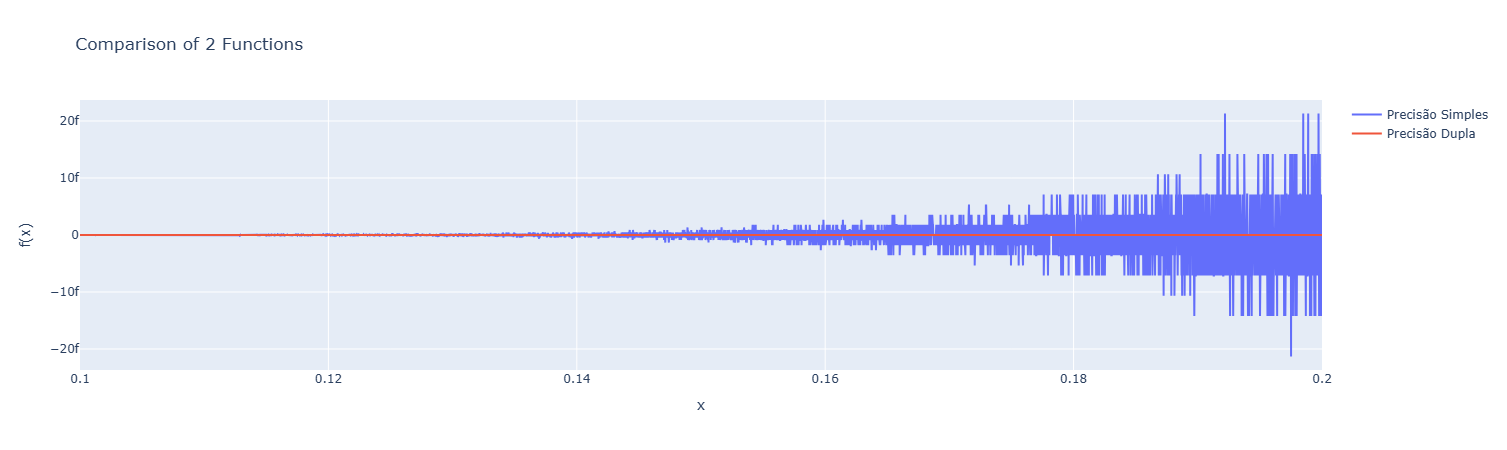
\includegraphics[width=1\textwidth]{Imagens/casosPeculiaresFP/timesXpot_literal0_1.png}
  \caption{Comportamento da expressão $f(x) = (x \times x \times x \times x \times x \times x \times x \times x \times x) - x^{10}$, com precisão simples, no intervalo \([0{,}1, 0{,}2]\).}
  \label{fig:timesXpot_literal0_1}
\end{figure}
A instabilidade na precisão dupla (Figura~\ref{fig:timesXpot_literal0_1}) produz imagem em torno de $[-4 \times 10^{-23},2 \times 10^{-23}]$, enquanto na precisão simples (Figura~\ref{fig:timesXpot_literal0}) está em torno de $[-20^{-15},20^{-15}]$ ($[-20 femto, 20 femto]$). Observa-se, portanto, que a diferença de instabilidade é extremamente menor na precisão dupla em comparação com a simples.

Uma outra situação é a diferença de como o computador interpreta algumas
funções se forem reescritas de maneiras diferentes. Seja $p(x) = (x - 1)^6$ e
$q(x) = x^6 - 6x^5 + 15x^4 - 20x^3 + 15x^2 - 6x + 1$, analiticamente essas
funções são idênticas, porém existem problemas de cancelamento catastrófico na
hora de analisarmos ambas em um sistema de ponto flutuante.

\begin{figure}[H]
  \centering
  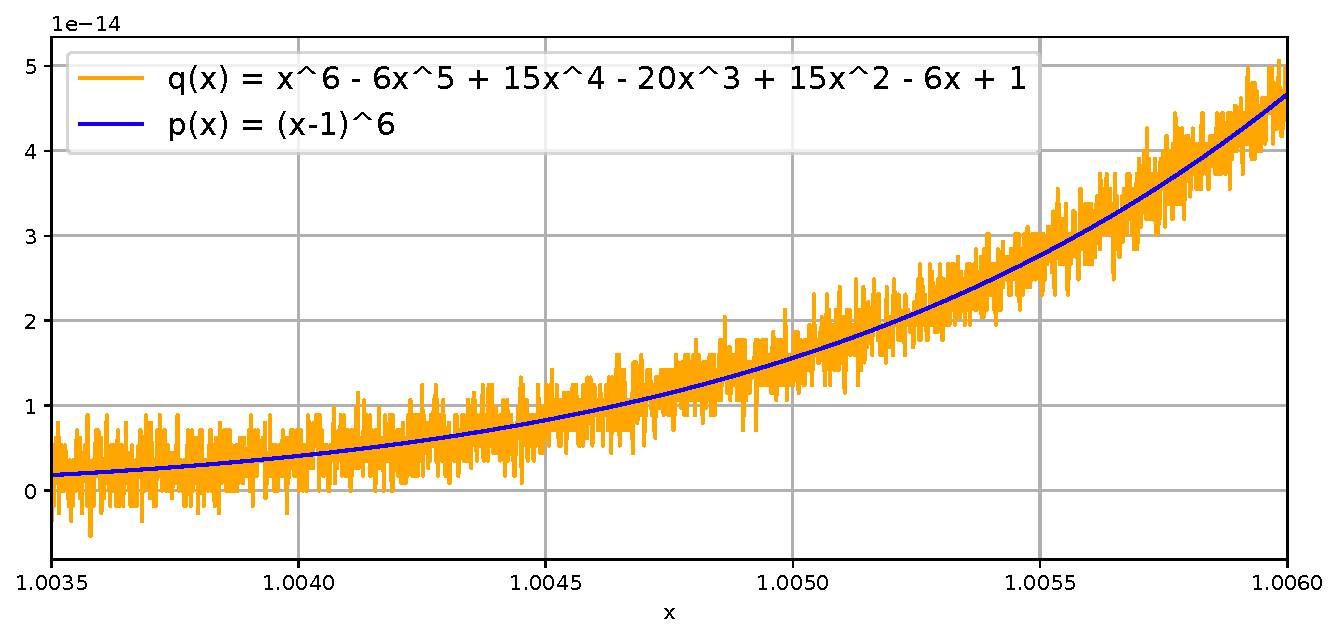
\includegraphics[width=1\textwidth]{Imagens/casosPeculiaresFP/NumError2_mplt}
  \caption{Comparação entre as funções $p(x) = (x - 1)^6$ e $q(x) = x^6 - 6x^5 + 15x^4 - 20x^3 + 15x^2 - 6x + 1$.}
  \label{fig:error2}
\end{figure}

\subsection{Discussão}

Esses exemplos destacam a importância da ordem das operações e da análise
cuidadosa ao trabalhar com algoritmos numéricos. Técnicas como a reordenação de
cálculos e o uso de formatos de precisão estendida podem ajudar a minimizar
esses erros em contextos críticos. Apesar de possivelmente surpreendentes,
esses fenômenos não invalidam a utilidade do ponto flutuante, pois o erro
observado tem ordem de grandeza muito pequena para a maioria das aplicações.
